\chapter{Programaci\'on objeto-funcional}
  Los lenguajes de programaci\'on emergentes de momento son aquellos
  que mezclan los conceptos de dos paradigmas presentes en la
  industria del software desde los a\~nos setenta, la orientaci\'on a
  objetos y la programaci\'on funcional.
\\
\\
  Mientras que la programaci\'on orientada a objetos se basa en
  abstracciones encapsuladas (los objetos) como base de su paradigma,
  la programaci\'on funcional se centra en las funciones como
  ciudadanos de primer orden.

\section{Programaci\'on orientada a objetos}

  La programaci\'on orientada a objetos ha sido inmensamente exitosa. 
  Empezando desde Simula en los a\~nos 60 y Smalltalk en los 70, es ahora el
  paradigma de programaci\'on predominante. El principio y
  motivaci\'on b\'asica de la programaci\'on orientada a objetos es
  simple: \emph{todos los programas requieren alg\'un tipo de
    estructura}\citep{programmingScala}.
\\
\\
  La forma mas simple de ejemplificarlo es a colocar datos y
  operaciones en algun tipo de contenedor. El concepto base de la
  orientaci\'on a objetos es hacer que estos contenedores sean
  generales, de forma que puedan contener datos y operaciones, y
  \'estos a su vez puedan ser contenidos en otros contenedores
  similares o que sean usados como par\'ametros para operaciones.
\\
\\
  Estos contenedores son denominados \emph{objetos}. Allan Kay, el
  inventor de Smalltalk, remarc\'o que de esta forma el objeto m\'as
  simple tiene el mismo principio de construcci\'on que un ordenador:
  \emph{combina datos con operaciones bajo una interfaz uniforme y
    formalizada}.  A pesar de que los lenguajes orientados a objetos
  han sido el foco de atenci\'on por mucho tiempo, existen
  relativamente pocos lenguajes que siguieron este principio b\'asico
  de construcci\'on hasta su conclusi\'on l\'ogica. 
\\
\\
  Por ejemplo,
  muchos lenguajes admiten valores que no son objetos, como los tipos
  de datos primitivos en Java. O permiten campos y operaciones
  est\'aticas que no son miembros de ning\'un objeto. \'Estas
  desviaciones del concepto original han conllevado a agregar
  complejidad y limitar escalabilidad en los
  programas\citep{programmingScala}.

\section{Programaci\'on funcional}

  Las ideas de programaci\'on funcional son m\'as antiguas que los
  ordenadores electr\'onicos. Sus fundamentos se remontan al c\'alculo
  lambda de la iglesia de Alonzo de los a\~nos 30. El primer lenguaje
  funcional fu\'e Lisp, creado en los a\~nos 50. Otros lenguajes
  funcionales populares son Scheme, SML, Erlang, Haskell, OCaml y
  F\#. Durante d\'ecadas la programaci\'on funcional ha estado
  limitada a campos acad\'emicos, sin embargo, en a\~nos recientes la
  industria de desarrollo ha incrementado su intere\'es en estos
  lenguajes\citep{programmingScala}.
\\
\\
  La programaci\'on funcional se gu\'ia por dos ideas:

  \begin{enumerate}
   \item Las funciones son valores de primer nivel.  \\ En un lenguaje
     funcional una funci\'on es un valor con la misma importancia que
     una cadena o un entero. Se pueden usar funciones como argumentos
     para otras funciones, retornar funciones como resultados o
     relacionarlas a con variables. Tambi\'en es posible definir
     funciones dentro de funciones de forma nominal o an\'onima.

   \item Las operaciones de un programa deber\'ian mapear valores de
     entrada hacia valores de salida si modificar el estado de los
     datos.
  \end{enumerate}

\section{Scala}

  Scala es un lenguaje de programaci\'on compatible con Java que ha
  estado en desarrollo desde el a\~no 2001 en el laboratorio de
  m\'etodos de programaci\'on del EPFL\footnote{\'Ecole Polytechnique
    F\'ed\'erale de Lausanne} y p\'ublicamente liberado para la
  plataforma JVM\footnote{Java Virtual Machine} desde Enero del 2004,
  la actual versi\'on estable es la 2.8 y es considerada como estable
  para ambientes de producci\'on.
\\
\\
  Scala combina programaci\'on orientada a objetos y funcional en un
  lenguaje est\'aticamente tipado. Est\'a orientado a la
  construcci\'on de componentes y sistemas de componentes desde su
  concepci\'on a trav\'es de los siguientes
  postulados\citep{scalaIntro}:

  \begin{itemize}
   \item Los lenguajes de programaci\'on para componentes de software
     necesitan ser escalables en el sentido de que los mismos
     conceptos pueden describir tanto partes grandes como peque\~nas
     de un sistema. Por tanto se concentra en mecanismos de
     abstracci\'on, composici\'on y decomposici\'on en vez de
     elementos primitivos que a pesar de ser \'utiles en cierta escala
     de bajo nivel no lo son a nivel de componentes.

   \item El soporte escalable para componentes puede ser prove\'ido
     por un lenguaje de programaci\'on que unifica y generaliza la
     programaci\'on funcional y la orientada a objetos.

  \end{itemize}
\subsection{Caracter\'isticas}

  Este es un resumen de los principales aspectos de
  Scala\citep{scalaIntro}:
  
  \begin{itemize}
   \item Scala combina la programaci\'on funcional y la orientada a
     objetos en un lenguaje uniforme.

   \item Los programas en Scala son similares a los programas en Java
     ya que Scala puede interactuar indistintamente con cualquier
     c\'odigo escrito en Java.

   \item Scala tiene un modelo de objetos uniforme, en el sentido de
     que cada valor es un objeto y cada operaci\'on una llamada de
     m\'etodo.

   \item Scala es a su vez un lenguaje funcional en el sentido de que
     las funciones son valores de primera clase.

   \item Scala tiene conceptos uniformes y poderosos para tipos de
     datos y valores.

   \item Scala tiene un sistema de construcci\'on de objetos y traits
     modular basado en la composici\'on flexible de mixins.

   \item Scala permite la descomposici\'on de objetos en base a la
     identificaci\'on de patrones.

   \item Scala permite extensiones externas de componentes usando
     vistas.

   \item Scala es un lenguaje est\'aticamente tipado, esto significa
     que el sistema clasifica variables y expresiones de acuerdo a los
     valores que pueden alojar y/o computar.

   \item Scala es compilado, todo c\'odigo escrito en Scala es
     compilado como bytecode completamente compatible con la m\'aquina
     virtual de Java.

   \item Scala est\'a dise\~nado como lenguaje de alto nivel, eso
     quiere decir que se enfoca en resolver problemas de forma
     productiva, reduciendo la complejidad a trav\'es del uso de
     niveles uniformes de abstracci\'on.

  \end{itemize}

  \begin{figure}[!hbtp]
    \centerline{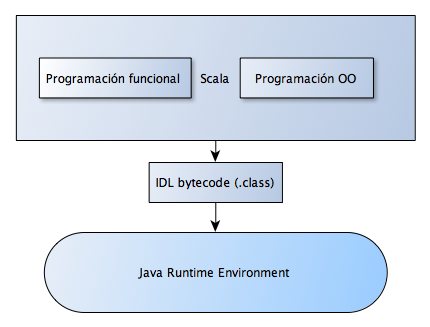
\includegraphics[height=7cm]{scala-overview.png}}
    \caption{Esquema general, Scala \citep{scalaIntro} }
  \end{figure}


%\subsection{Modelo de Objetos unificado}
%  TODO

\subsubsection{Clases y objetos}

  Las clases son notaciones est\'aticas que permiten definir elementos 
  con atributos, operaciones y estados. Los objetos son elementos 
  instanciados a partir de una clase, por ejemplo, el objeto Neo es 
  instancia de la clase Humano.
  
  Scala permite definir las clases de forma simplificada, una clase
  Java se definir\'ia as\'i:

  \begin{mylisting}
  \begin{verbatim}
  class MyClass {
      private int index;
      private String name;

      public MyClass(int index, String name) {
        this.index = index;
        this.name = name;
      }
    }
  \end{verbatim}
  \end{mylisting}

  y su equivalente en Scala es:

  \begin{mylisting}
  \begin{verbatim}
    class MyClass(index: Int, name: String)
  \end{verbatim}
  \end{mylisting}

  Y agrega un nuevo tipo de dato denominado \emph{objeto}, que es 
  un tipo de dato de instancia \'unica en el entorno de ejecuci\'on.

  \begin{mylisting}
  \begin{verbatim}
    object FindLongLines {
      def main(args: Array[String]) {
        val width = args(0).toInt
        for (arg <- args.drop(1))
          LongLines.processFile(arg, width)
        }
    }
  \end{verbatim}
  \end{mylisting}

\subsubsection{Funciones y m\'etodos}

  Las funciones son secuencias de \'ordenes ejecuci\'on 
  que tienen valores de entrada y salida, los m\'etodos son
  funciones que est\'an contenidas dentro de objetos. 

  Ya que la programaci\'on funcional define a las funciones 
  como elementos de primer orden, las funciones pueden ser parte 
  de otras funciones, ya sea de forma determin\'istica o an\'onima.

  \begin{mylisting}
  \begin{verbatim}
    def processFile(filename: String, width: Int) {
      def processLine(filename: String, width: Int, line: String) {
        if (line.length > width)
          println(filename +": "+ line)
      }
      val source = Source.fromFile(filename)
      for (line <- source.getLines()) {
        processLine(filename, width, line)
      }
    }
  \end{verbatim}
  \end{mylisting}
%\subsubsection{Variables y propiedades}
%  TODO
%\subsection{Operaciones}
%  TODO
%\subsubsection{M\'etodos y valores funcionales}
%  TODO
%\subsubsection{Funciones}
%  TODO
%\subsection{Abstracci\'on}
%  TODO
%\subsubsection{Abstracciones funcionales}
%  TODO
%\subsubsection{Miembros abstractos}
%  TODO
%\subsection{Composici\'on}
%  TODO
